\documentclass[a4paper,12pt]{article}
\usepackage[pdftex]{graphicx}
\usepackage[T1]{fontenc}
\usepackage[utf8]{inputenc}
\usepackage{lmodern}
\usepackage[sort, numbers]{natbib}
%\usepackage{graphicx}
\usepackage{amsmath}
\usepackage{soul}

\title{Temperature and energy measurements in ultra-low temperature Helium-3}
\author{P. Franchini}

\begin{document}

\maketitle
%\tableofcontents

%\begin{abstract}
%\end{abstract}

\section{Bolometric model for energy measurement}

Specific heat capacity $C_V$ as a function of the temperature $T$ (in units of [J/K/m$^3$]) has been calculated from the entropy of a system of independent fermions, quasiparticles~\cite{vollhardt}, as

\begin{equation}
C_V(T)=2(2\pi)^{1/2}k_BN_0\varDelta\left(\frac{\varDelta}{k_BT}\right)\exp\left(-\frac{\varDelta}{k_BT}\right)
\end{equation}

where $k_B$ is the Boltzmann constant, $N_0$ is the density of quasiparticle states in the normal phase at Fermi energy for one spin component, $\varDelta$ ($\approx 1.76 k_B T_c$ at 0\,bar) is the average gap energy at low temperature near the critical temperature for superfluidity $T_c$ ($\simeq$930\,$\mu$K at 0\,bar). They all depend on pressure P.

$C_V(T)$ has a strong dependency with temperature (fig.~\ref{fig:CvT})

\begin{figure}[htb]
  \begin{center}
    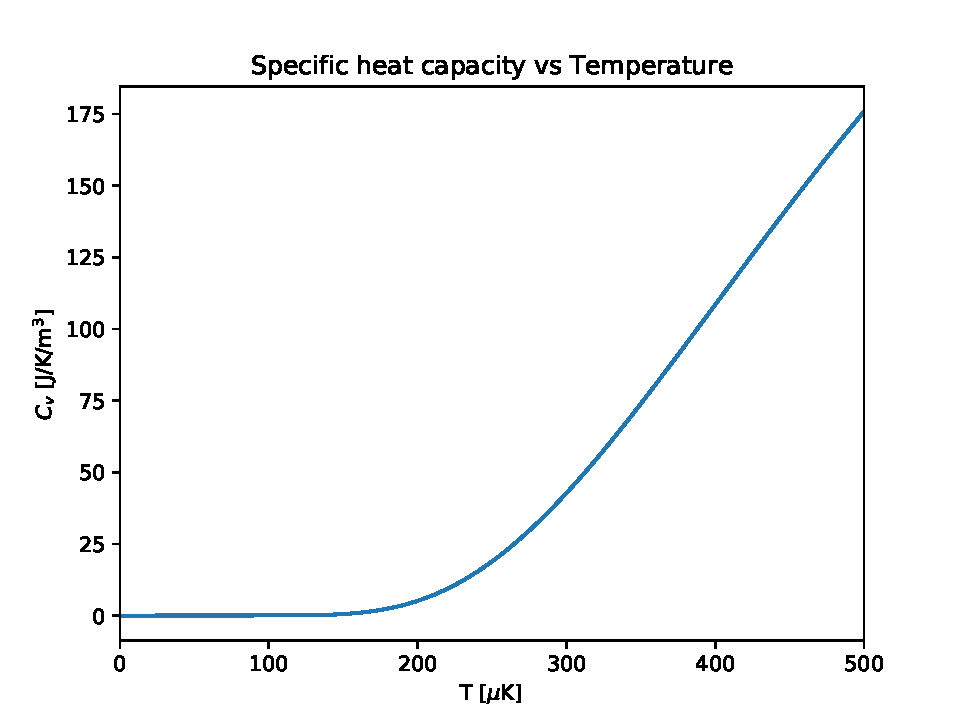
\includegraphics[width=0.69\textwidth]{Cv_vs_T-zoom}
  \end{center}
  \caption{$C_V$ vs T, below $T_c$. He3 has an extremely low heat capacity at low temperatures.}
  \label{fig:CvT}
\end{figure}

To obtain the heat variation $\Delta Q$ between two temperatures $T_1$ and $T_2$ for a a given volume $V$ of helium-3 is required the integration

\begin{align}
\Delta Q (T_1,T_2) = \Delta C_V V & = V \int_{T_1}^{T_2} C_V(T)dT \\
                                  & = V \left( \int_{0}^{T_2} C_V(T)dT - \int_{0}^{T_1} C_V(T)dT \right)\\
                                  & = V \left( I(T_2) - I(T_1) \right)  
\end{align}

where

\begin{align}
I(T) = \int_{0}^{T} C_V(T)dT & = \sqrt{2} \pi N_0 \varDelta^2 \left( 1 - \frac{2}{\sqrt{\pi}}\int_{0}^{\sqrt \frac{\varDelta}{k_BT}} e^{-t^2} dt \right) \\ 
                             & =  \sqrt{2}\pi N_0\varDelta^2 \mathrm{erfc} \sqrt{\frac{\varDelta}{k_BT} } 
\end{align}

therefore

\begin{equation}
\Delta Q (T_1,T_2) = \sqrt{2}\pi N_0\varDelta^2 \left( \mathrm{erfc}\sqrt{\frac{\varDelta}{k_BT_2}} - \mathrm{erfc}\sqrt{\frac{\varDelta}{k_BT_1}} \right)V
\end{equation}

We consider the 1\,cm$^3$ volume of helium-3 at a certain base temperature $T_0$ so we can calculate the temperature variation $\Delta T$ for an energy deposition $\Delta Q(T_0,T_0+\Delta T)$;
since both $N_0$ and $\varDelta$ are function of the pressure we calculate the energy deposition for 4 different pressures in the range (0--30)\,bar (fig.~\ref{fig:TDE})

\begin{figure}[!ht]
  \begin{center}
  \begin{tabular}{cc}
    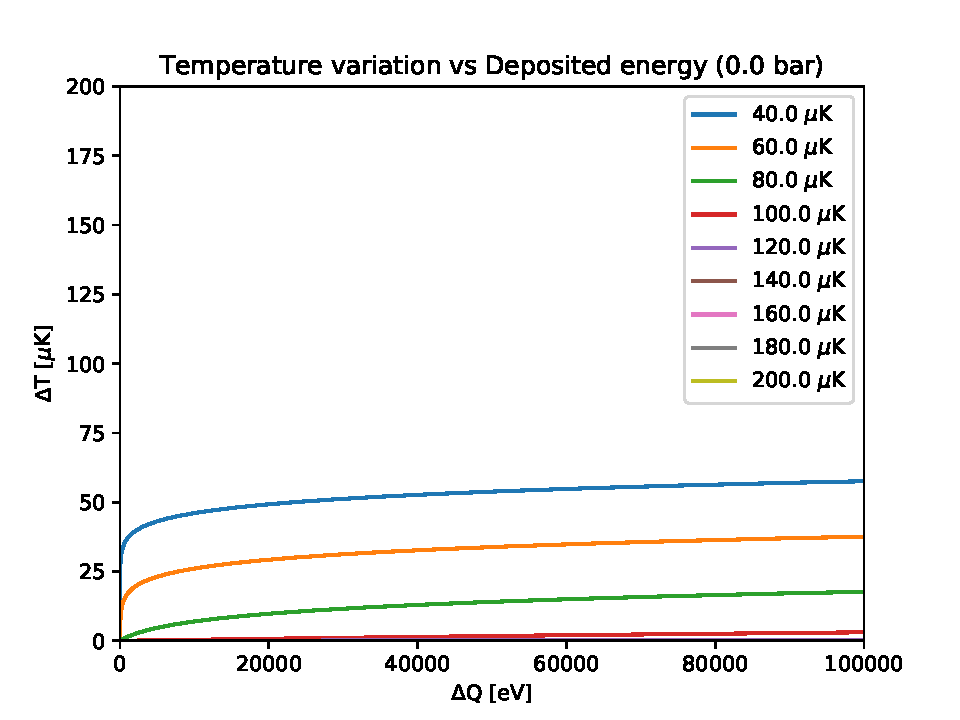
\includegraphics[width=0.49\textwidth]{T_vs_DE-0bar} &
    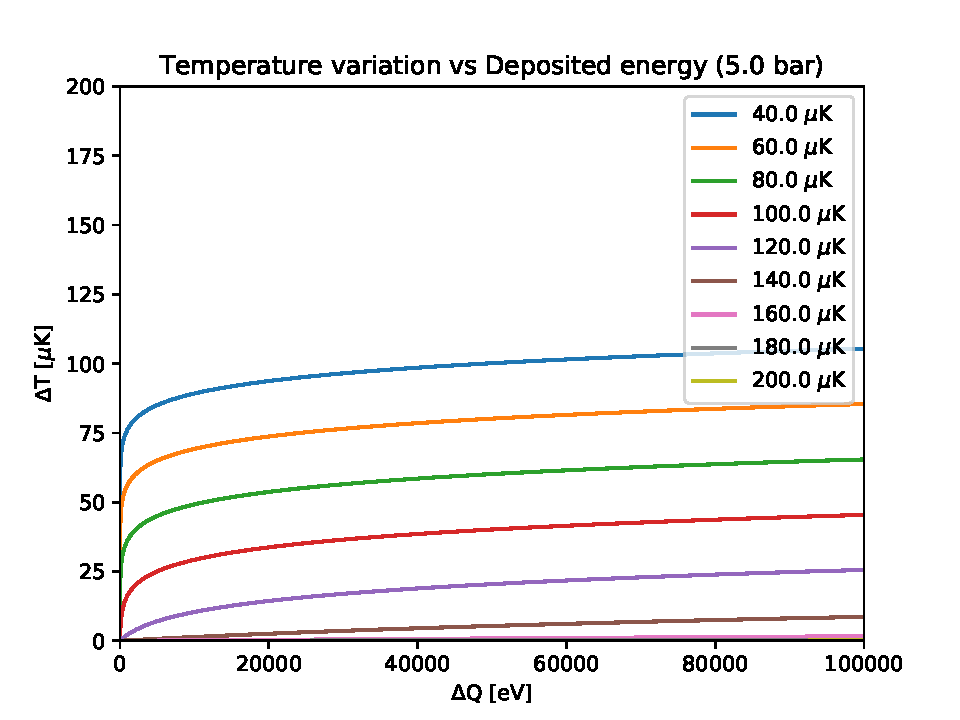
\includegraphics[width=0.49\textwidth]{T_vs_DE-5bar} \\
    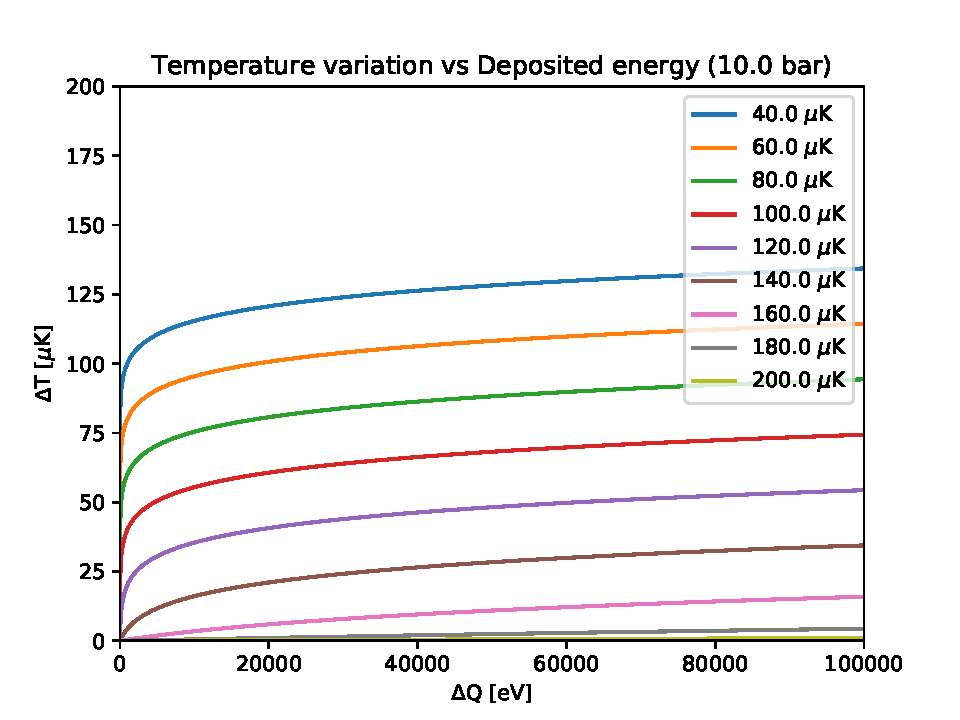
\includegraphics[width=0.49\textwidth]{T_vs_DE-10bar} &
    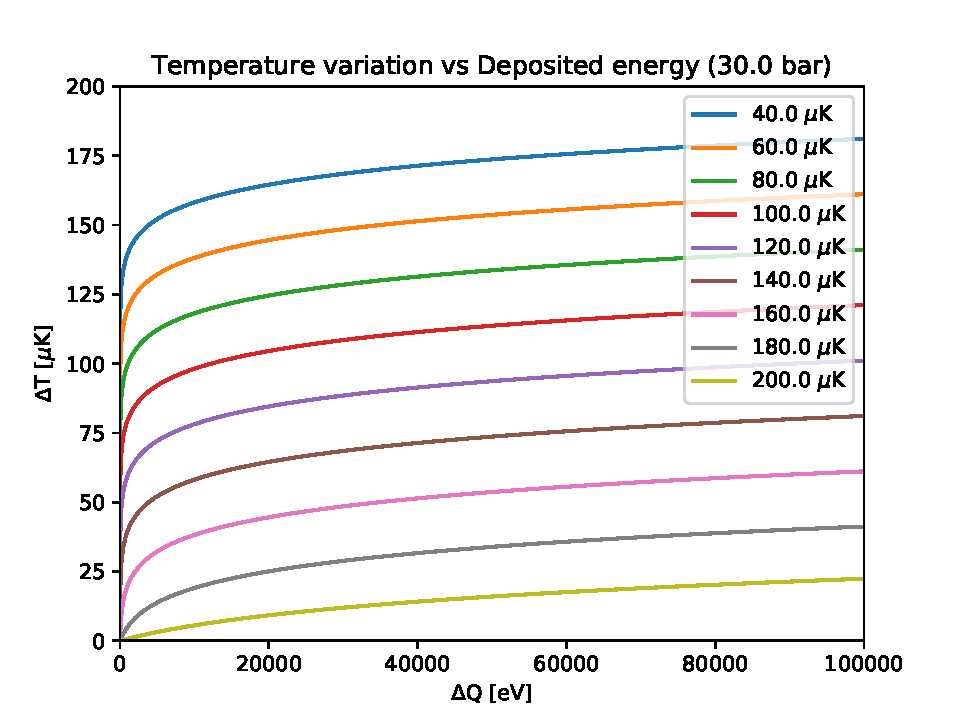
\includegraphics[width=0.49\textwidth]{T_vs_DE-30bar}
  \end{tabular}
  \end{center}
  \caption{$\Delta T$ vs $\Delta Q$ for several $T_0$ in the range 40--200\,$\mu$K for pressures of 0\,bar (top-left), 5\,bar (top-right), 10\,bar (bottom-left), 30\,bar (bottom-right).}
  \label{fig:TDE}
\end{figure}

Higher pressures for higher system temperatures have equivalent effects in terms of temperature variations.

For a vibrating wire resonator (VWR), either from an amplitude sweep or a resonance tracking is possible to calculate the \textit{resonance width} $\Delta f$ which can be used to infer the temperature~\cite{lawson}.
Since the resonance width is
\begin{equation}
\Delta f = \frac{2F}{\pi \rho d}
\end{equation}

where $d$ and $\rho$ are respectively the diameter and the mass density of the wire, and $F$ is the damping %(?)
force (in units of length, velocity and diameter), defined as

\begin{equation}
F = \frac{\pi}{4}p^2_F v_F N_0 \exp{\left( -\frac{\varDelta}{k_B T} \right)}
\end{equation}

The resonance width expressed in terms of temperature is

\begin{equation}
  \Delta f = \frac{p^2_F v_F N_0}{2\pi\rho d}\exp{\left( -\frac{\varDelta}{k_B T} \right)}
  \label{eq:width}
\end{equation}

e.g. in fig.~\ref{fig:WvsT} for a Niobium-Titanium wire of 150\,nm diameter in a volume at 1\,bar; therefore the temperature can be derived from the resonance width

\begin{figure}[!ht]
  \begin{center}
    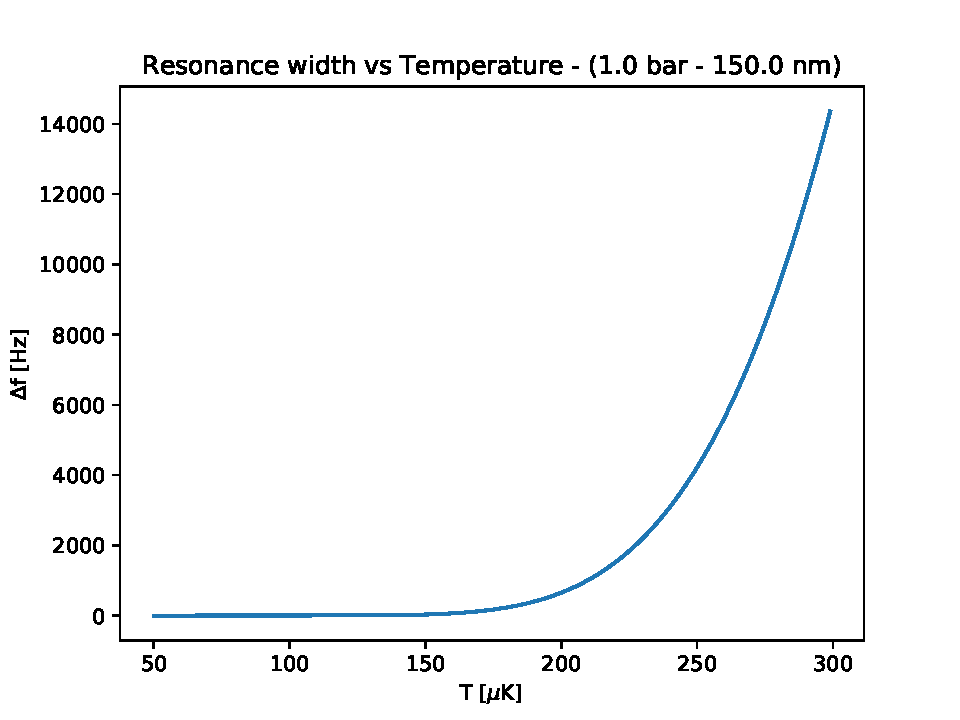
\includegraphics[width=0.69\textwidth]{W_vs_T}
    \caption{Resonance frequency width dependence on temperature for a nano-wire.}
    \label{fig:WvsT}
  \end{center}
\end{figure}

\begin{equation}
T = - \frac{\varDelta}{k_B \ln \left( \Delta f \frac{2 \pi \rho d}{p_F^2 v_F N_0} \right)}
\end{equation}

The increase of resonance width $\Delta (\Delta f)$ in response of an energy deposition $\Delta Q$ is linearly proportional, as shown in figures~\ref{fig:DeltaDeltaWvsDE} and \ref{fig:DeltaDeltaWvsDE-wire}.
The constant of proportionality is inversely proportional to the base temperature (and pressure), so the other way around, in terms of energy deposition
\begin{equation}
  \Delta Q = \alpha(T_0,P) \Delta (\Delta f), \alpha \propto T_0
    \label{eq:alpha}
\end{equation}

\begin{figure}[!ht]
  \begin{center}
  \begin{tabular}{cc}
    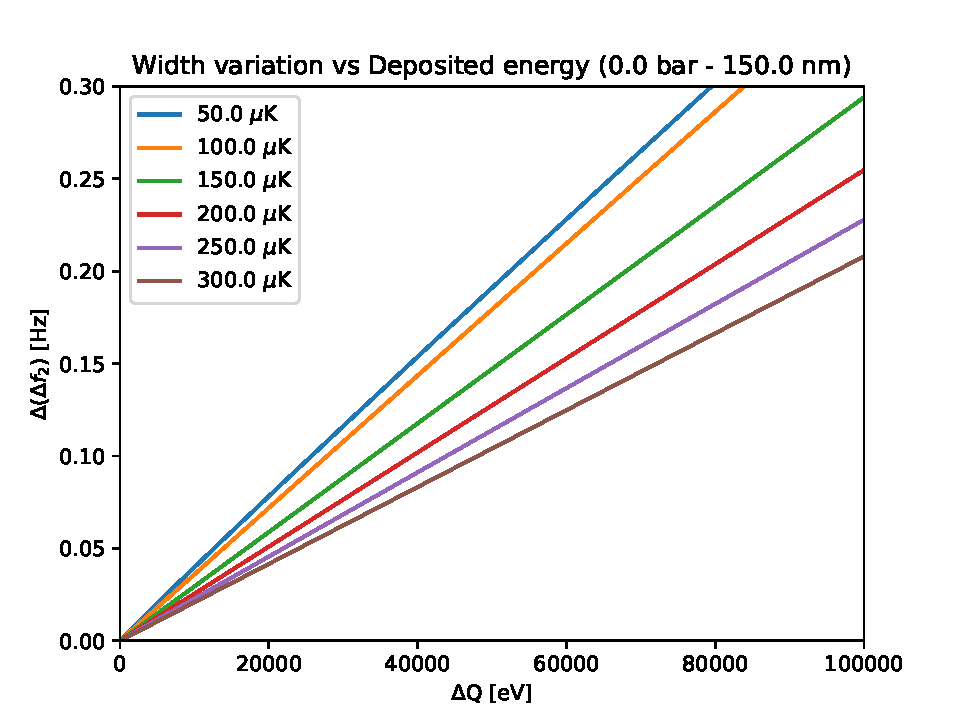
\includegraphics[width=0.49\textwidth]{DeltaDeltaW_vs_DE-0bar}  &
    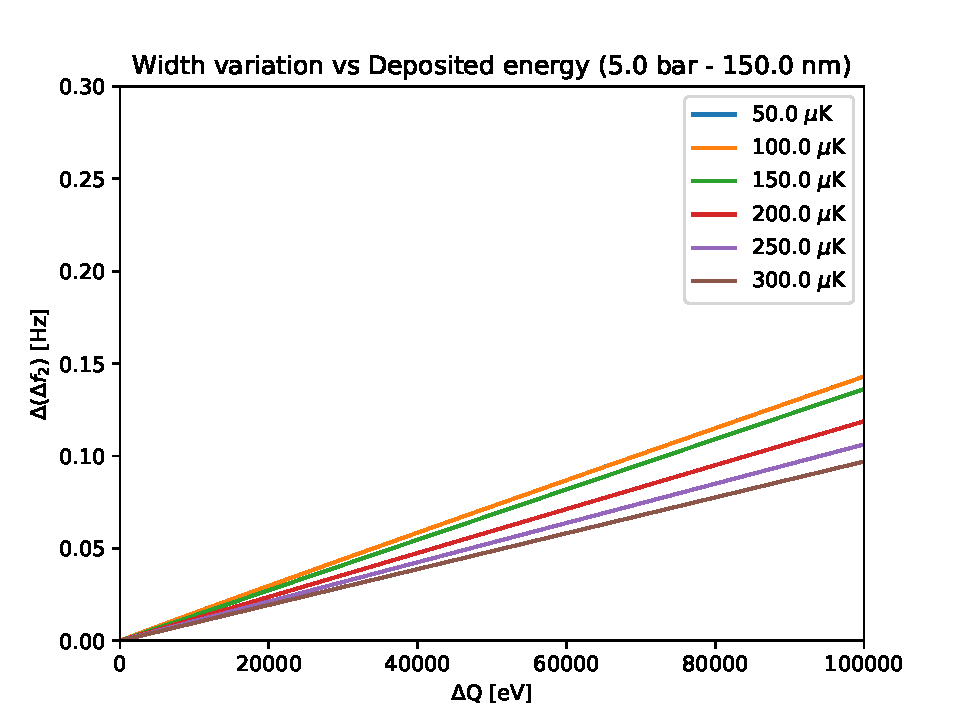
\includegraphics[width=0.49\textwidth]{DeltaDeltaW_vs_DE-5bar}  \\
    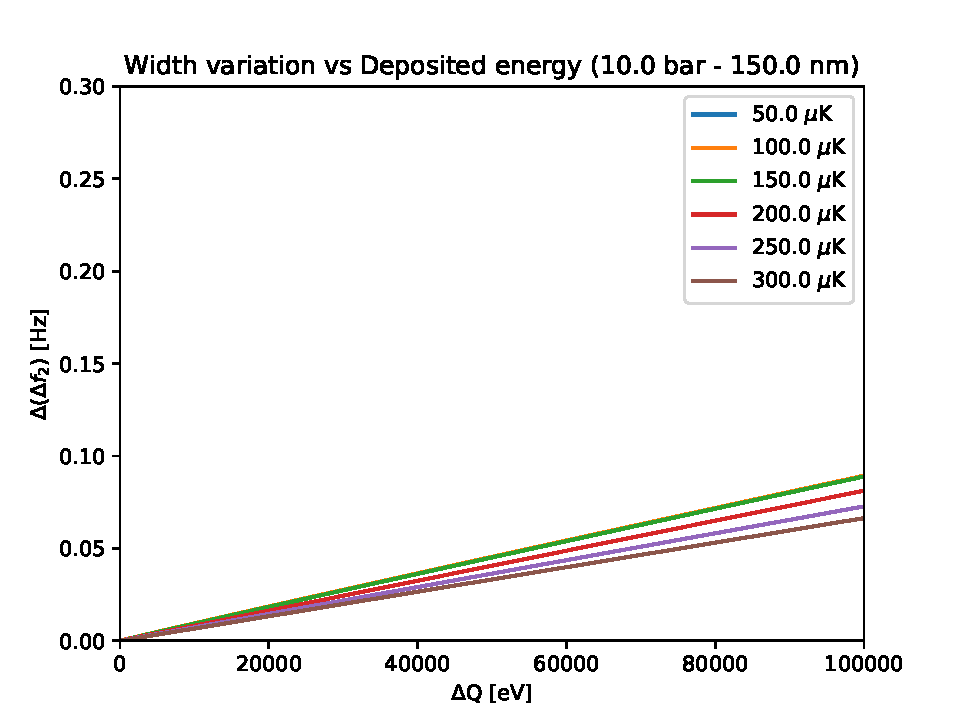
\includegraphics[width=0.49\textwidth]{DeltaDeltaW_vs_DE-10bar} &
    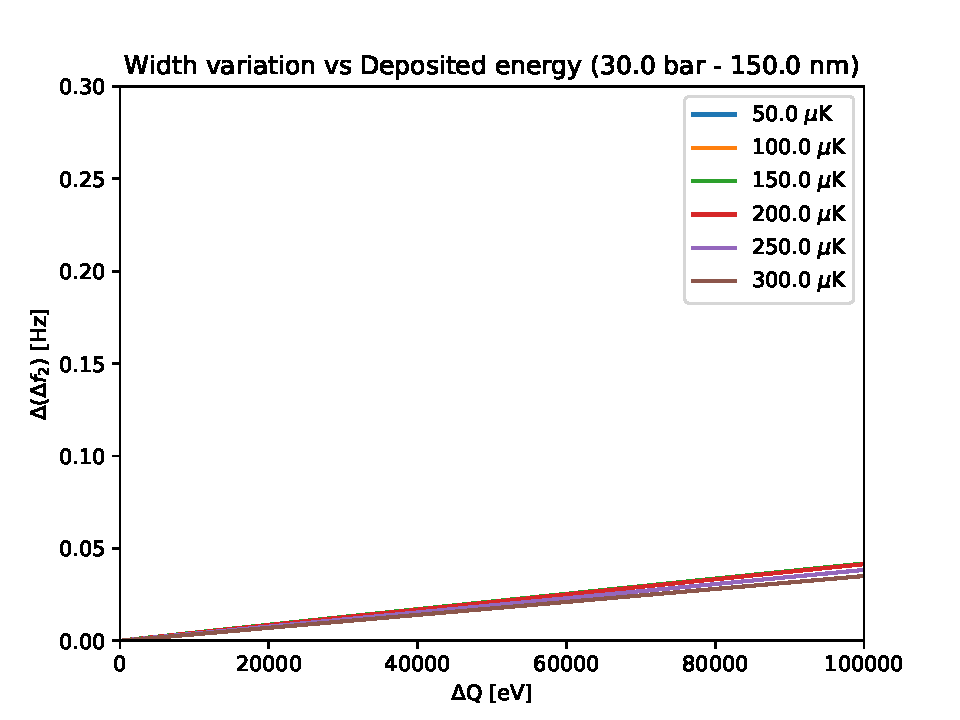
\includegraphics[width=0.49\textwidth]{DeltaDeltaW_vs_DE-30bar}
  \end{tabular}
  \end{center}
  \caption{$\Delta(\Delta f)$ vs $\Delta Q$ for several $T_0$ in the range 50--300\,$\mu$K for pressures of 0\,bar (top-left), 5\,bar (top-right), 10\,bar (bottom-left), 30\,bar (bottom-right).}
  \label{fig:DeltaDeltaWvsDE}
\end{figure}

\begin{figure}[!ht]
  \begin{center}
  \begin{tabular}{cc}
    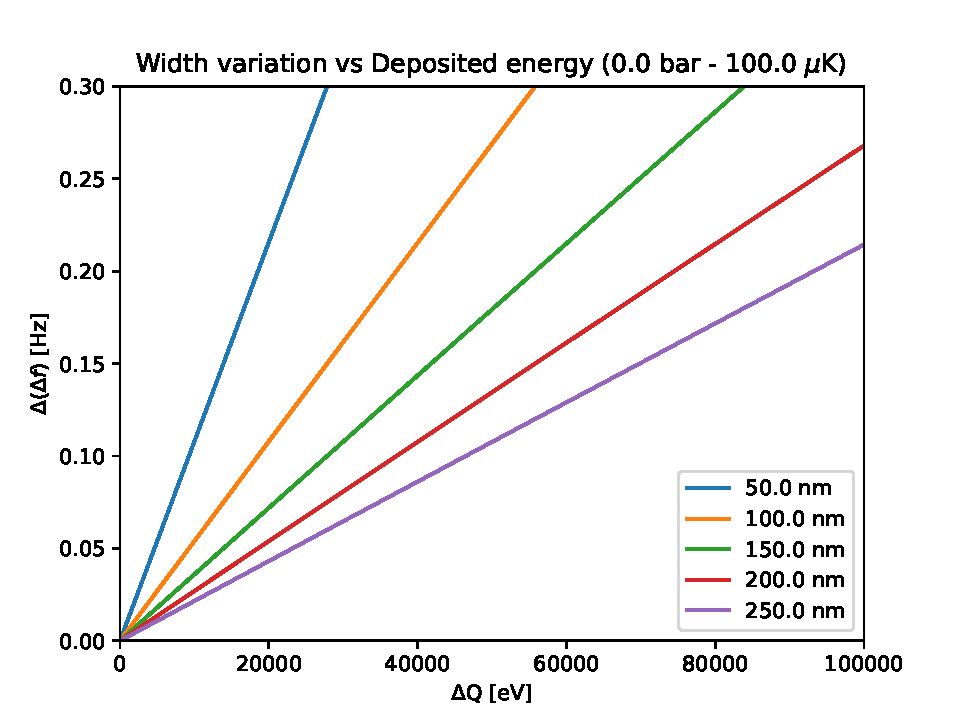
\includegraphics[width=0.49\textwidth]{DeltaDeltaW_vs_DE_wire-0bar}  &
    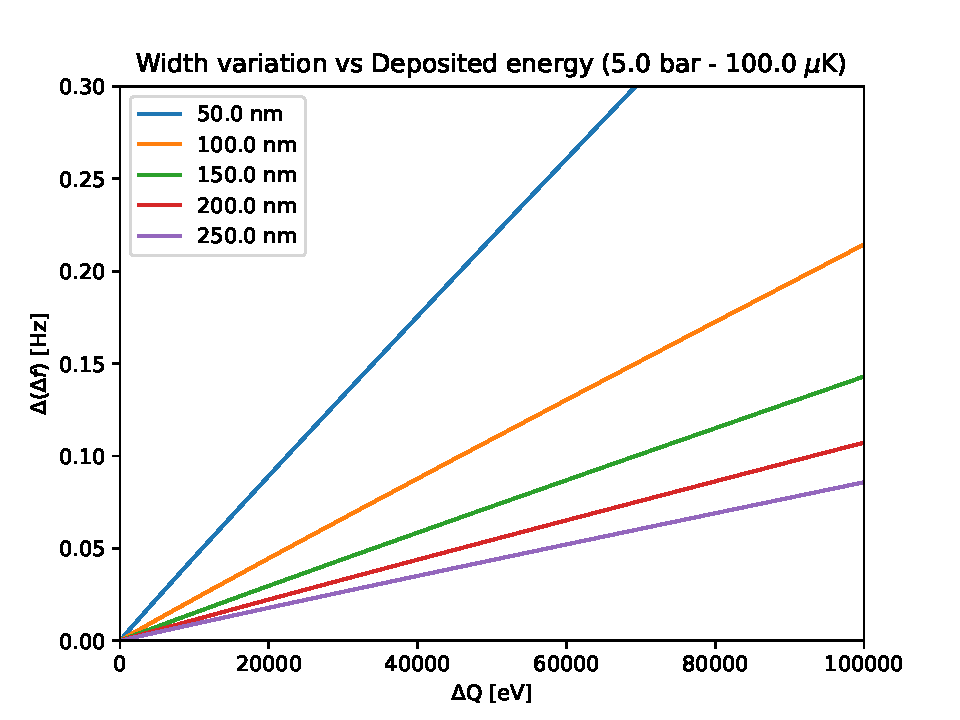
\includegraphics[width=0.49\textwidth]{DeltaDeltaW_vs_DE_wire-5bar}  \\
    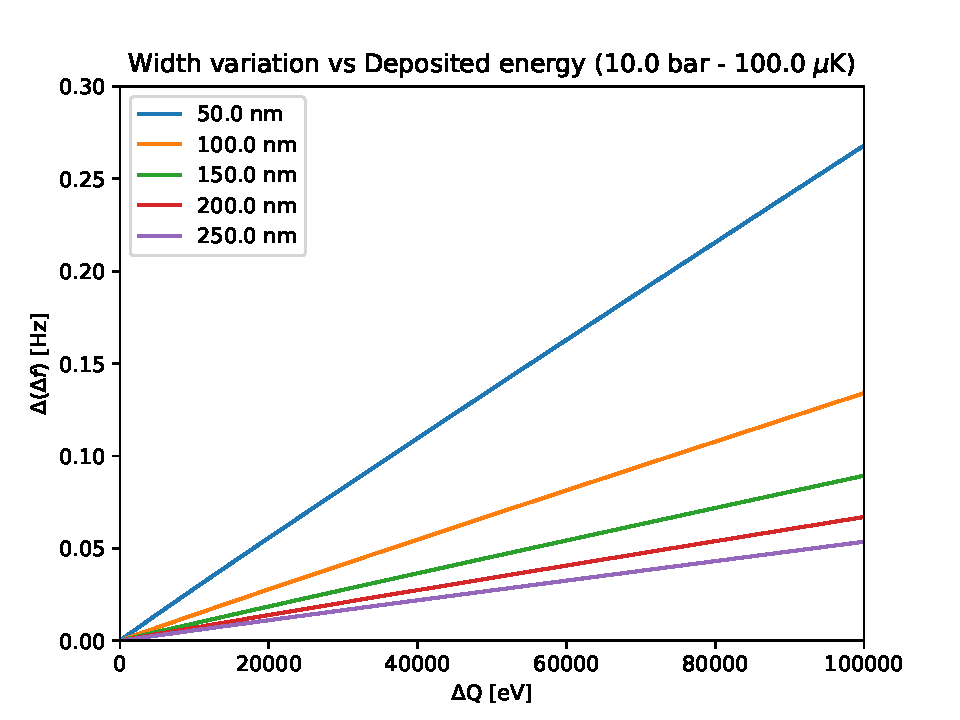
\includegraphics[width=0.49\textwidth]{DeltaDeltaW_vs_DE_wire-10bar} &
    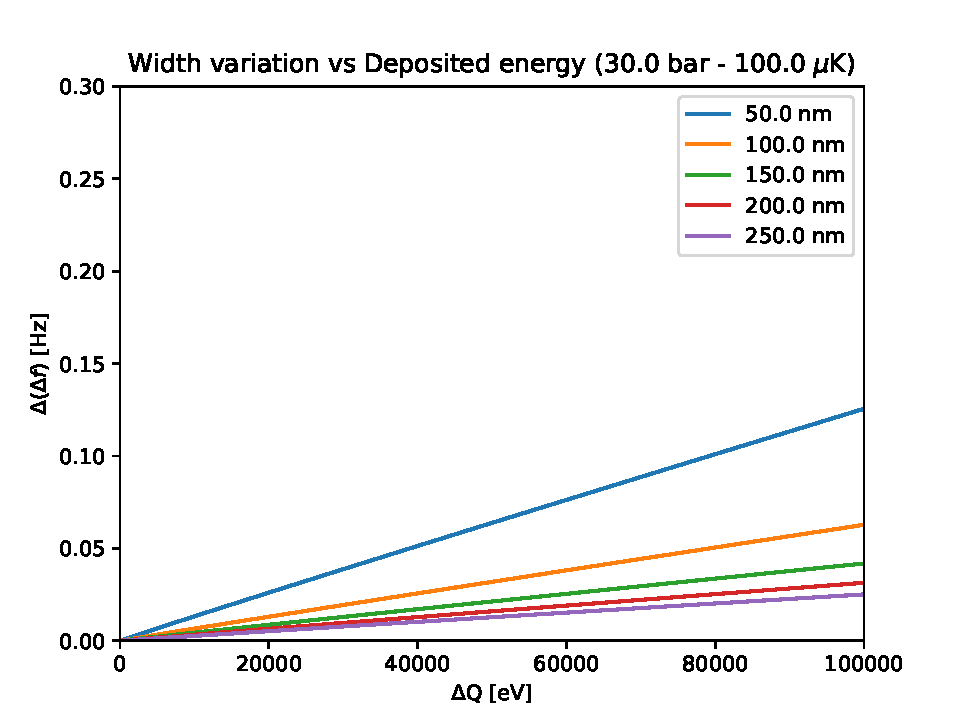
\includegraphics[width=0.49\textwidth]{DeltaDeltaW_vs_DE_wire-30bar}
  \end{tabular}
  \end{center}
  \caption{$\Delta(\Delta f)$ vs $\Delta Q$ for several wire diameters in the range 50--250\,nm for pressures of 0\,bar (top-left), 5\,bar (top-right), 10\,bar (bottom-left), 30\,bar (bottom-right).}
  \label{fig:DeltaDeltaWvsDE-wire}
\end{figure}

The increase of resonance width $\Delta (\Delta f)$ can be measured from fitting each bolometric recorded event, e.g. in figure~\ref{fig:winkelmann} from~\cite{winkelmann},
\begin{figure}[!ht]
  \begin{center}
    \begin{tabular}{cc}
    \includegraphics[width=0.42\textwidth]{winkelmann} &
    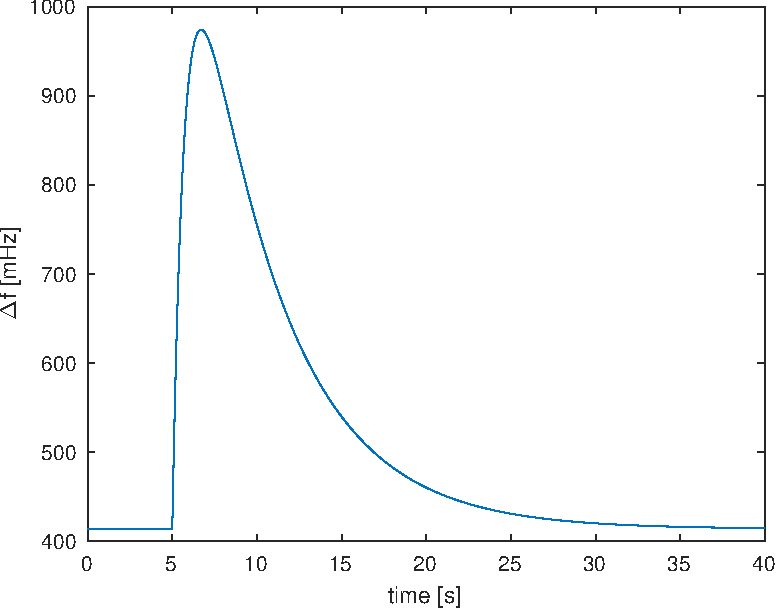
\includegraphics[width=0.49\textwidth]{winkelmann_fit.pdf}
    \end{tabular}
  \end{center}
  \caption{Example of an energy deposition event for a 4.5\,$\mu$m wire in a volume of 0.14\,cm$^3$ of He-3. H in the paper's notation is proportional to $\Delta (\Delta f)$ with respect to a base width~\cite{winkelmann} (\textit{left}); fit function as in eq.~\ref{fit} (\textit{right}) with $\tau_b$=5\,s, $\tau_w$=0.77\,s and $\Delta f_\mathrm{base}$=414\,mHz.}
  \label{fig:winkelmann}
\end{figure}
using the function

\begin{equation}
  \Delta f(t)= \Delta f_\mathrm{base} + \Delta (\Delta f) {\left( \frac{\tau_b}{\tau_w} \right)}^{\tau_w/(\tau_b-\tau_w)} \frac{\tau_b}{\tau_b - \tau_w} \left( e^{-t/\tau_b} - e^{-t/\tau_w} \right)
\label{fit}
\end{equation}

(which is derived for $\tau_b \neq  \tau_w$) in order to extract the maximum variation $\Delta (\Delta f)$, where $\Delta f_\mathrm{base}$ is the base width at the base temperature of the helium, $\tau_w$ is the response time of the oscillating wire
\begin{equation}
  \tau_w \simeq \frac{1}{\pi \Delta f} = \mathrm{const}
\end{equation}
and $\tau_b$ is the decay constant, proportional to the Kapitza resistance (the thermal boundary resistance limiting the heat conduction between the solid metal and the liquid helium)
\begin{equation}
  \tau_b = R_K(T) C_V
\end{equation}
Note that the energy measurement depends only on $\Delta (\Delta f)$ and not on the response time and decay constant.
%is not necessary to fit the peak pulse.

Considering that there are three main variables, base temperature, pressure of the helium, wire diameter (considering fixed the wire material and the helium volume), all with an interplay between each other, we can at least extract few conclusions:
\begin{itemize}
  \item For small wires there is a higher amplitude of the width response $\Delta (\Delta f)$. In other terms the \textit{sensitivity} increases reducing the wire diameter (as $1/d$), as in figure~\ref{fig:SensitivityVsDiameter}.
  \item For low temperatures there is an higher amplitude of the width response $\Delta (\Delta f)$
  \item For high pressures there is a lower width response for a certain energy deposition
  \item The response time of the oscillating wire is faster for high temperatures 
  \item The decay time of the oscillating wire is faster for high temperatures (low Kapitza resistance), so low temperatures might cause some pile-up of events
\end{itemize}

\subsection{Sensitivity dependence}

If we define the sensitivity as the width variation per deposited energy.....

\begin{figure}[!ht]
  \begin{center}
    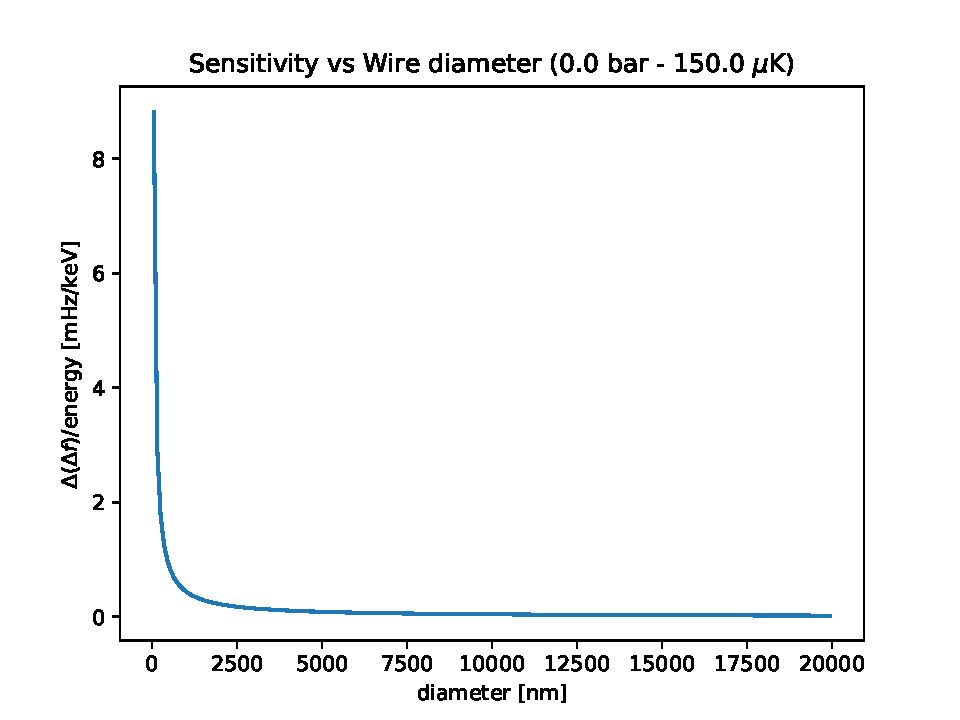
\includegraphics[width=0.69\textwidth]{Sensitivity_vs_diameter-0bar}
    \caption{Sensitivity measuring the deposited energy with width variation vs wire diameter.}
    \label{fig:SensitivityVsDiameter}
  \end{center}
\end{figure}



% ============================================

\section{Laboratory readout}

Ultimately the actual method of measurement performed in the lab is done in terms of voltage readout of the oscillating wire, in two main steps:
\begin{enumerate}

  \item \textit{Sweep measurement} to extract the resonance frequency of the wire for a certain base temperature and the base width $\Delta f_\mathrm{base}$. The quantities are extracted from the Lorentzian fits of the in-phase and out-of-phase signal (Voltage vs Frequency). This should provide the error $\sigma_{\Delta f_\mathrm{base}}$.
  \item Data acquisition with the setup sitting at the resonance frequency (\textit{resonance tracking}) for a fixed voltage drive value $V_D$ (amplitude of the injected voltage). The measurement is voltage height $V_H$. From the Lorentzian function we know that
  \begin{equation}
    \frac{V_H\Delta f}{V_D} = \mathrm{const} = K
  \end{equation}
in particular for the base values at the steady state (before the heat pulse)
  \begin{equation}
    \frac{V_{H_\mathrm{base}}\Delta f_\mathrm{base}}{V_D} = \mathrm{const} = K
  \end{equation}
so we are going to measure $\Delta f(t)$, as in figure~\ref{fig:winkelmann}, as
  \begin{equation}
    \Delta f(t) = \frac{V_D}{V_H(t)}K = \frac{V_{H_\mathrm{base}} \Delta f_\mathrm{base}}{V_H(t)}
  \end{equation}
  
\end{enumerate}

% ============================================

\section{Errors}

In order to answer to the following questions, we need to find which is the measurement uncertainty coming from the laboratory setup:
\begin{itemize}

  \item What is the minimum voltage variation we can measure, hence the threshold of the energy deposition? 
  \item Which is the resolution in the resonance width variation (aka temperature variation), hence the resolution of the energy deposition?

\end{itemize}

We assume that the main uncertainty comes from the voltage measurement $\sigma_{V_H}$ which propagates into the determination of $\Delta f_\mathrm{base}$
and into the quality of the fit to extract $\Delta (\Delta f)$

The error on the energy deposition should be

\begin{equation}
  \sigma_{\Delta Q}  \simeq \left| \frac{\partial \Delta Q}{\partial(\Delta(\Delta f))} \right| \sigma_{\Delta (\Delta f)} \overset{\mathrm{eq. \ref{eq:alpha}}}{=} \alpha (T_0,P) \sigma_{\Delta (\Delta f)}
\end{equation}

The analytical error propagation might prove to be ineffective; is worth assigning an error coming from the voltage measurement noise from the lock-in amplifier and do a systematic error study starting from a toy distribution generated $\Delta f(t)$ (where the noise is present both for the baseline and for the signal distribution); find an error on the fit done to extract $\Delta (\Delta f)$; propagate this error to $\Delta Q$.

Since the data acquisition will fit $\Delta f$ we need to add the uncertainty $\sigma_{\Delta f}$ on the toy generated function from eq.~\ref{fit}, where
\begin{equation}
\sigma^2_{\Delta f}(t) = \left( \frac{\partial \Delta f(t)}{\partial V_H(t)} \right)^2 \sigma^2_{V_H} + \left( \frac{\partial \Delta f(t)}{\partial \Delta f_\mathrm{base}} \right)^2 \sigma^2_{\Delta f_\mathrm{base}} = \left( \frac{(\Delta f(t))^2}{V_{H_{\mathrm{base}}} \Delta f_\mathrm{base}} \right)^2 \sigma^2_{V_H} + \left( \frac{\Delta f(t)}{\Delta f_\mathrm{base}}\right)^2 \sigma^2_{\Delta f_\mathrm{base}}
\end{equation}
if we consider only the error on the voltage measurement $\sigma_{V_H}$ (while the error on the base frequency $\sigma_{\Delta f_\mathrm{base}}$ would need to be determined by a separate toy simulation on the Lorentzian fit for the amplitude sweep)
\begin{equation}
\sigma_{\Delta f}(t) = \left| \frac{\partial \Delta f(t)}{\partial V_H(t)} \right| \sigma_{V_H} = \frac{(\Delta f(t))^2}{V_{H_{\mathrm{base}}} \Delta f_\mathrm{base}} \sigma_{V_H}
\end{equation}
producing a distribution like in~figure~\ref{fig:toy}. To summarize the independent parameters present in the simulation are

\begin{itemize}
  \item volume and pressure of the helium-3 cell (V, P)
  \item wire density ($\rho$)
  \item diameter of the oscillating wire (d)
  \item base temperature of the helium ($T_0$)
  \item decay constant $\tau_b$ \st{and response time $\tau_w$}
  \item base voltage height ($V_{H_\mathrm{base}}$)
  \item error on the voltage measurement ($\sigma_{V_H}$)
\end{itemize}

\begin{figure}[!ht]
  \begin{center}
    \begin{tabular}{cc}
    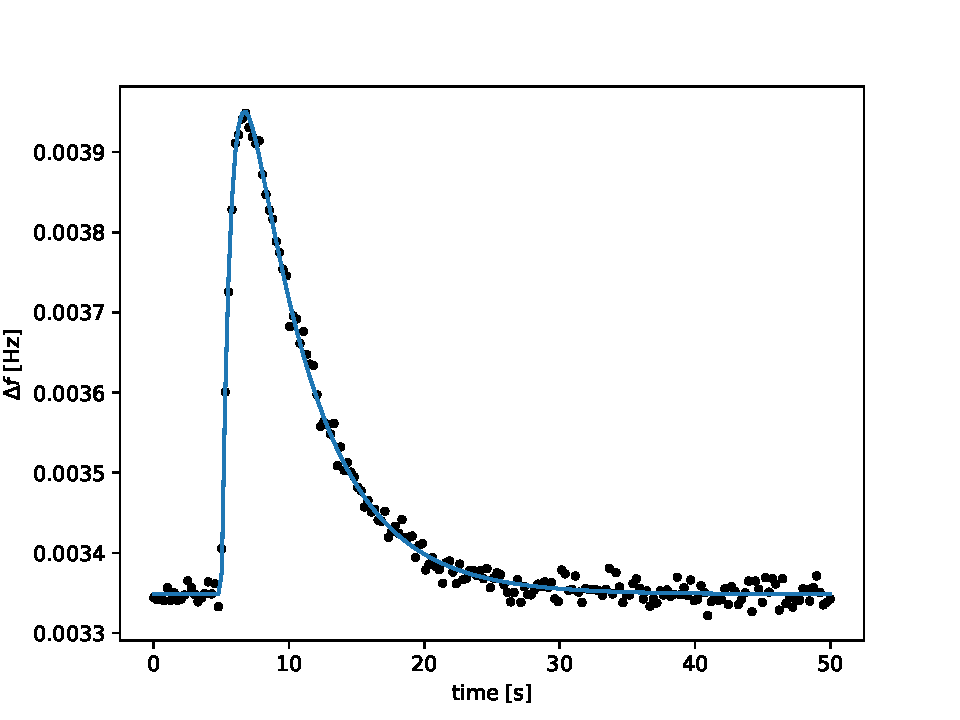
\includegraphics[width=0.49\textwidth]{deltaf_toy-example} &
    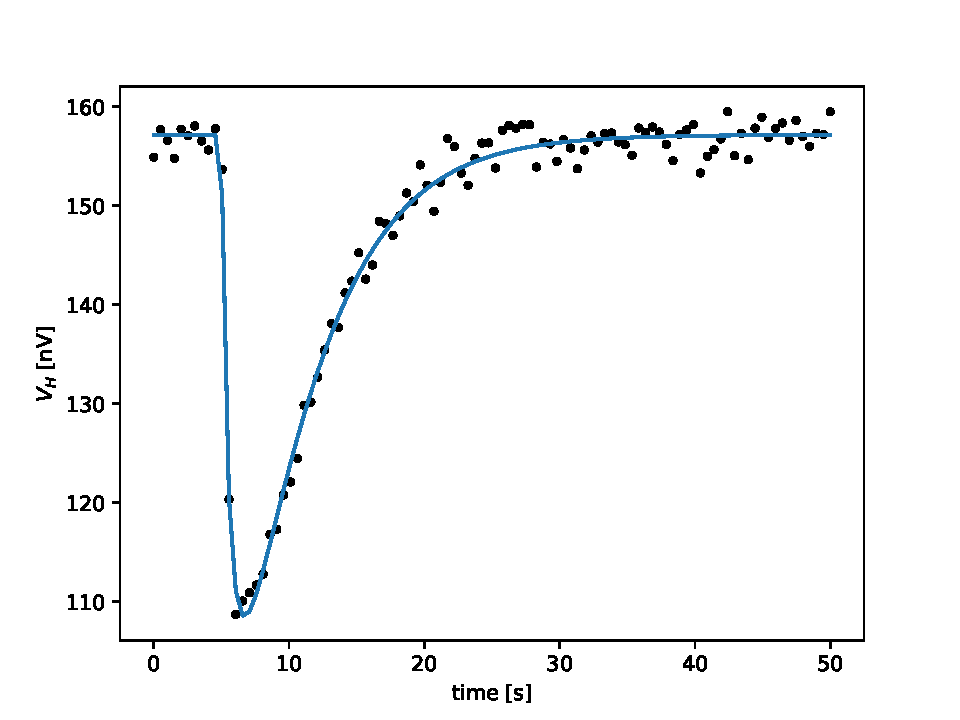
\includegraphics[width=0.49\textwidth]{voltage_toy-example}
    \end{tabular}
    \caption{Example of a pseudo-experiment distribution of $\Delta f(t)$ (\textit{left}) and $V_H(t)$ (\textit{right}).}
    \label{fig:toy}
  \end{center}
\end{figure}

The randomization and fit of the pseudo-experiments is repeated N times, ultimately extracting the distribution of the deposited energy from the fitted $\Delta(\Delta f)$ using eq.~\ref{eq:alpha}, as in figure~\ref{fig:energy_distribution}.

\begin{figure}[!ht]
  \begin{center}
    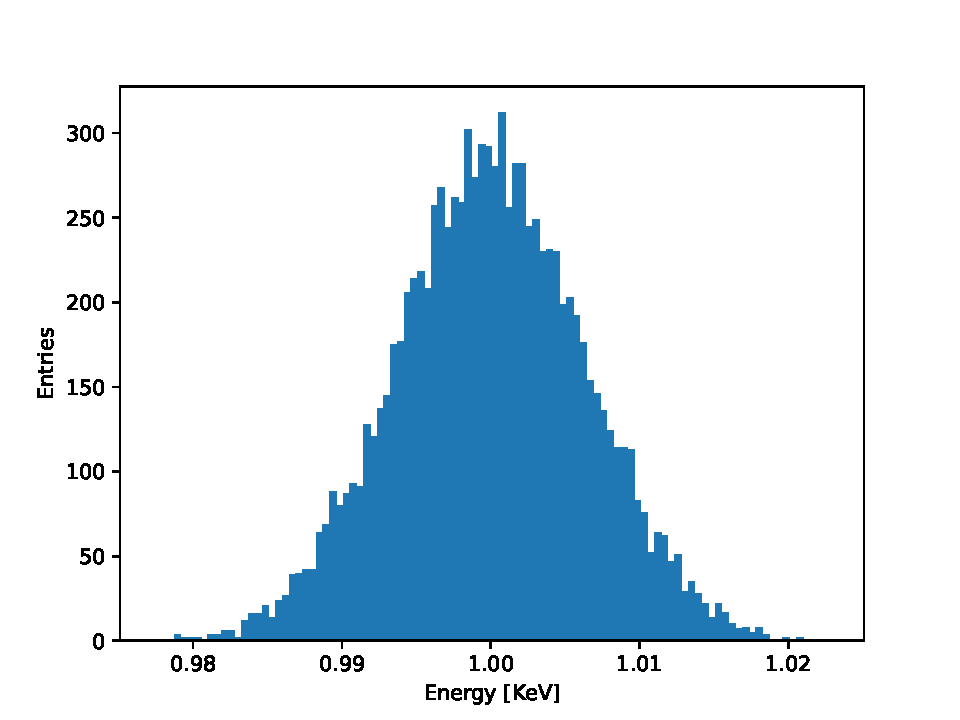
\includegraphics[width=0.69\textwidth]{energy_distribution}
    \caption{Energy distribution for 10000 toys.}
    \label{fig:energy_distribution}
  \end{center}
\end{figure}

The error for the energy measurement can be related to $\sigma/\mu$, so for a range of energies [0--100]\,keV is possible to obtain distributions of the expected error for a certain configuration (figure~\ref{fig:error})

\begin{figure}[!ht]
  \begin{center}
    \begin{tabular}{cc}
    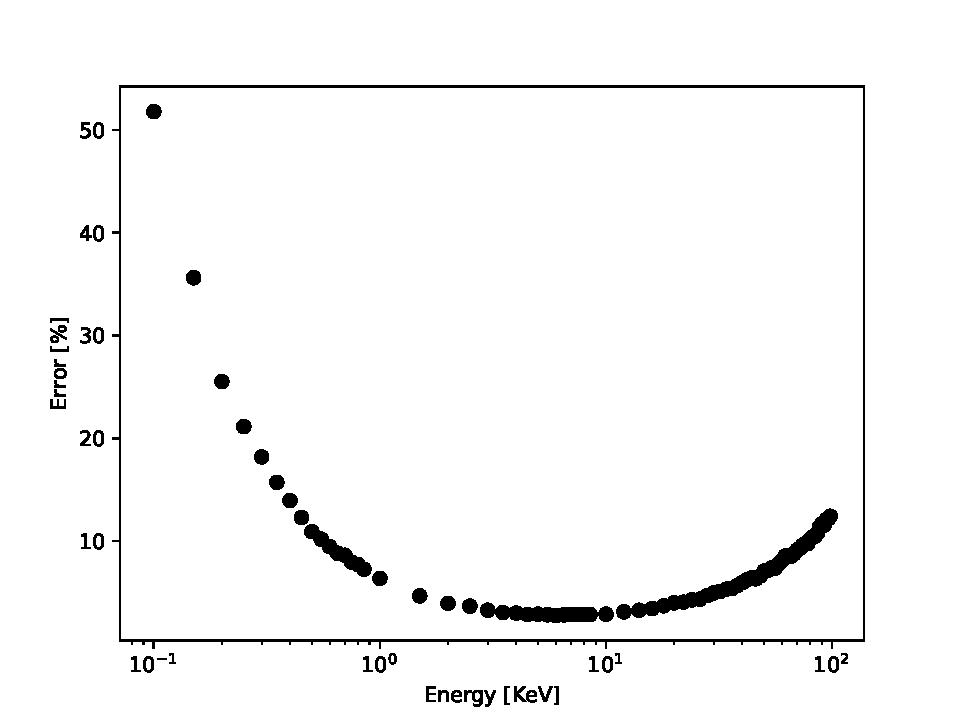
\includegraphics[width=0.49\textwidth]{error_200nm}
    \end{tabular}
    \caption{Error vs energy (in a certain configuration), for a 200\,nm wire. The relative error increases with high energies because is proportional to the square of the width increase.}
    \label{fig:error}
  \end{center}
\end{figure}

In order to consider the error on the wire diameter we should take into account also the error on the base width, so

\begin{align}
  \sigma_{\Delta Q}^2 & \simeq \left( \frac{\partial \Delta Q}{\partial \Delta f_\mathrm{base}} \right)^2 \sigma_{\Delta f_\mathrm{base}}^2 
                             + \left( \frac{\partial \Delta Q}{\partial(\Delta(\Delta f))} \right)^2 \sigma_{\Delta (\Delta f)}^2  \\
                      & = \left( \frac{\partial \alpha}{\partial \Delta f_\mathrm{base}} \biggr\rvert_{(T_0,P)} \Delta(\Delta f )\right)^2 \sigma_{\Delta f_\mathrm{base}}^2
                        + \alpha^2(T_0,P) \sigma_{\Delta (\Delta f)}^2
\end{align}

where the derivative of the slope $\alpha$ can be approximated as

\begin{align}
  \frac{\partial \alpha}{\partial \Delta f_\mathrm{base}} & \simeq
  \frac{\alpha(\Delta f_\mathrm{base}+\delta/2) - \alpha(\Delta f_\mathrm{base}-\delta/2) }{\delta} = \\
       & = \frac{\alpha(T_0+\delta/2) - \alpha(T_0-\delta/2) }{\delta} \frac{\partial T(\Delta f)}{\partial \Delta f} = \\
       & = \frac{\alpha(T_0+\delta/2) - \alpha(T_0-\delta/2) }{\delta} \frac{k_B}{\varDelta} \frac{T^2}{\Delta f(T)}
\end{align}

We can define the base voltage $V_{H_{\mathrm{base}}}$ fixing the wire velocity to $v$=1\,mm/s, assuming a field $B$=100\,mT and a leg spacing $D$=2\,mm, according to this, describing the induced voltage of the wire moving in a magnetic field as
\begin{equation}
V_H(t) = \frac{\pi}{4} B D v(t)
\end{equation}
(where the geometrical constant $\pi/4$ corresponds to a semi-loop), $V_{H_{\mathrm{base}}} \simeq 157\,nV$ 


\section{SQUID readout}
We consider the circuit noise as

\begin{equation}
V_{RMS}  = \sqrt{\big|Z(\omega_0) + R + i\omega_0 L_i\big|^2 S_\phi \Delta f / M_i^2 + 4 k_B T R \Delta f + k_B T l B^2 / m}
\end{equation}

so the error on the voltage measurement, rescaled for the bandwidth $B = \pi f_\mathrm{base}/2$ corresponding to the base width is

\begin{equation}
\sigma_{V_H} = \frac{V_{RMS}}{B}\sqrt{f_{NEP}} = \frac{V_{RMS}}{\sqrt{\pi f_\mathrm{base}/2}} \sqrt{\mathrm{0.250 \cdot \pi f_\mathrm{base}/2}}
\end{equation}



\section{Readout}

We can study the position of the peak of the energy deposition pulse as in figure \ref{fig:winkelmann}; considering the pulse starting at $t=0$, the maximum correspond to
\begin{equation}
t' = \frac{\tau_b \tau_w}{\tau_w - \tau_b} \ln \frac{\tau_w}{\tau_b}
\end{equation}
so it depends on the decay constant and on the response time (which depends on the base width).
A wire too fast will not be read in time, so the minimum should coincide with the time constant of the readout.
A wire too slow would cause some pile-up of events, if the maximum time is slower than the reciprocal of the rate of events.

The rate of events is dominated by the background. The most relevant contribution comes from cosmic rays and cosmic rays induced background, which can be up to one event per minute in absence of any shielding or tagging.

Likely the peak would need to be within a fraction of a second and 10 seconds.
This is compatible with a hundred nano-meter wire, operated a zero pressure with a relative temperature of 0.1. A thicker wire would require a higher pressure



\section{Quasiparticle shot-noise}

The temperature dependent quasiparticle number density $n$ is

\begin{equation}
%n = \frac{m^* p_F}{\pi \hbar^2}k_B T \exp \left( {-\frac{\Delta}{k_BT}} \right) \\
n = \frac{1}{\pi^2} \left( \frac{2m^*}{\hbar^2} \right) ^{3/2} \sqrt{E_F} k_B T \exp \left( {-\frac{\Delta}{k_BT}} \right) \\
\end{equation}
where $E_F = p_F^2/(2m^*)$~\cite{vonka}.\\
As a two dimension approximation, a flux $N=\frac{1}{2}nv_FDa$ of quasiparticles of effective mass $m^*$ impacts on a wire of length $D$ and radius $a$, from one direction.\\
The distribution of QP hitting the wire follows a Poisson distribution, therefore the error (input \textit{shot-noise}, or spectral noise) corresponds to the standard deviation $\sqrt{N}/\sqrt{\mathrm{Hz}}$:
%in a bandwidth $B$

\begin{align}
\sigma_N &= \sqrt{N} = \sqrt{\frac{nv_FDa}{2B}}
\end{align}
therefore the relative error (aka \textit{fractional noise}) per $\sqrt{\mathrm{Hz}}$ is
\begin{equation}
  \sqrt{N}/N = \frac{1}{\sqrt{N}} = \sqrt{\frac{2}{n v_F D a}}
\end{equation}
so the shot-noise becomes relevant for a low fluxes (low temperatures), because the quasiparticle flux on the wire reduces as the temperature, so the fluctuation of the QP density becomes important~\cite{bradley}.

Rewriting eq.~\ref{eq:width} in terms N gives
\begin{equation}
  \Delta f = N \frac{\pi p_F N_0 \hbar^3}{8 \rho a D m^* k_b T}
\end{equation}
Therefore the error relative to the shot-noise in a bandwidth B is
\begin{equation}
  \sigma_{\Delta f} = \frac{\partial \Delta f}{\partial N} \sigma_N \sqrt{B} = \frac{\Delta f}{N}\sqrt{N} \sqrt{B} = \frac{\Delta f}{\sqrt{N}} \sqrt{B}
\end{equation}
or
\begin{equation}
  \sigma_{\Delta f} = \frac{\partial \Delta f}{\partial N} \sigma_N \sqrt{f_{NEP}} = \frac{\Delta f}{N}\sqrt{N} \sqrt{B} = \frac{\Delta f}{\sqrt{N}} \sqrt{f_{NEP}}
\end{equation}
which can be used to calculate the uncertainty in the energy measurement determined by the pure shot-noise.

As bandwidth of $\pi f_\mathrm{base}/2$ is used.

% ============================================

\pagebreak
\newpage

\begin{thebibliography}{9}

\bibitem{vollhardt} Vollhardt, D., Wolfle, P., The Superfluid Phases of Helium 3 (1990)
\bibitem{lawson} Lawson, C.R., A Novel Measurement Device for use in Multiphase Helium-3 and 4 at Ultra-Low Temperatures, MPHys thesis (2014)
\bibitem{winkelmann} Winkelmann et al, Bolometric calibration of a superfluid 3He detector for Dark Matter search: Direct measurement of the scintillated energy fraction for
neutron, electron and muon events (2007)
\bibitem{lev} Lev, L., SQUID readout of a vibrating nanowire (2022)
\bibitem{bradley} D. I. Bradley and W. M. Hayes, An RF-SQUID Amplifier System for Use with Vibrating Wire Resonators (1999)
\bibitem{vonka} J. Vonka, Demagnetisation of Solid 3He \& Supercritical Superflow, thesis, 2018
\end{thebibliography}

\end{document}
